\documentclass[11pt]{article}
\usepackage{hyperref}

%\usepackage{fontspec}
%\defaultfontfeatures{Mapping=tex-text}
%\setmainfont{Linux Libertine O}
%\setsansfont{Linux Biolinum O}
%\setmonofont{DejaVu Sans Mono}

\usepackage{hyperref}
\hypersetup{unicode=true, colorlinks, breaklinks, citecolor=blue, linkcolor=black}

\usepackage{xltxtra}
\usepackage{booktabs} 
\usepackage{subfigure}
\usepackage{graphicx}

\setcounter{secnumdepth}{4}

\title{An Emperical Analysis on User Interests on GitHub}
\author{Jiacheng Pan}

\begin{document}
\maketitle

\section{Introduction}
GitHub is a very popular platform for developing software in collaboration nowadays. At the same time, with many features provided by the website, such as following a user, starring and forking a repository, people can use GitHub as an information platform to share and obtain new ideas all over the globe.

In this paper, investigations are made to explore 1) how users' interest towards repositories looks like; 2) how repositories are related to each other based on the context of users' interest; 3) how users' interest as well as the relationship between repositories change over time.

\section{Related Work}
Some recent works have examined the conditional probablities as well as the correlations between programming languages used by users and the language pairs \cite{doll12,shah13}.

Also based on GitHub, the relatioship between repository collaboration networks has been examined and visualized, in accordance with the programming languages being used \cite{ford13,marrama}.

User communities based on primary programming languages and ``follower'' relationships were explored in \cite{cuny10,weber12}.  A visualization of the bipartite graph of organizations (groups of users) and languages \cite{rodrigues12} won third place in the 2012 GitHub Data Challenge.  

Important nodes in the one-mode project-project and user-user networks, weighted simply by number of common links, were identified in \cite{thung2013}.

Also recent models of network evolution capturing the growth process incorperating 1) constant average degree assumption; 2) slowly growing diameter assumption are discussed in \cite{albert1999internet,broder2000graphStructure,Watts-Colective-1998}.

\section{Data Set}
\subsection{Data Collection}
GitHut published their timeline data since 2012 at www.githubarchive.org \cite{githubarchive}, and the same datasets are as well queryable via Google BigQuery \cite{googlebigquery}, through which all the raw data used in this paper are collected. 
In particular, the space of public watch events, i.e. starring a repository when people finds it interesting, on GitHub between January 2012 to October 2014 are collected and aggregated every quarter.
At the same time, the main language used and the accumulated star number of each repository of interest are collected.
In order to reduce computational complexity, only the watch events towards the repositories that have more than 1000 accumulated stars by the end of each quarter are collected.

\subsection{Repository Interest Graph}
In order to explore how users' interest may look like, this paper tries to observe a graph with repositories being the nodes, while the count of starring users of both repositories being the edges. 

Through this graph, which is derived from a bipartite graph between users and repositories, it may be easy to find out what else repositories may be liked by users when a certain repository is starred. And therefore to further estimate the relationship between repositories based on such an interest context.

In detail, we define graph nodes as the repositories being starred, when the repository has more than 1000 accumulated stars by the end of each quarter.
Also, we connect two nodes, i.e. repositories, when a user has starred both of the repositories within the same quarter. And the total number of such users is marked as the edge weight.

Since we intend to explore how the repository interest graph may change over time, eleven such graphs are built thoughout the timeline data, snapshotting users' behaviours within each quarter.

\section{Analysis}
\subsection{Static Observation}
In this section, a snapshot network is analyzed, by viewing the layout and colouring of the graph, as well as by using network metrics.

\subsubsection{Visual Analysis}
We first select the Y13Q2 (Year 2013, Quarter 2nd, April 2013 -- June 2013) dataset to analysis a network snapshot of the repository interest graph.

Using Gephi, with the Force Atlas layout algorithm, the graph is shown in figure \ref{fig:static_community}, coloured with Moduality Class cacluated by Gephi, and sized in accordance to the accumulated star number of the repositories by the end of the quarter. At the same time, the same graph is shown in figure \ref{fig:static_lang} using language colouring, i.e. colouring the repositories regarding the main language they use.

Comparing these two plots, it is easy to find out that the community distribution correlates with the language.
And from this observation, it is also understandable to deduct that people are likely to star repositories of languages they are famaliar with.

Also from the both plots, the Objective-C cluster stands out of the main cluster, forming a relatively lonely community (figure \ref{fig:zoom_2013}). This shows 1) users who likes objective-c repositories are likely to be interested in objective-c repositories themselves; 2) users who likes objective-c repositories are less likely to be interested in Ruby or VimL (the purple nodes near the Ruby cluster) or PHP, and so on.
And therefore we may further guess that objective-c users may be more distant and isolated from the world of web programming, which involves languages like Ruby, PHP, and Javascript etc., in terms of their interests.

\begin{figure}[htp!]
  \subfigure[Dataset Y13Q2, coloured with Moduality Class] { 
    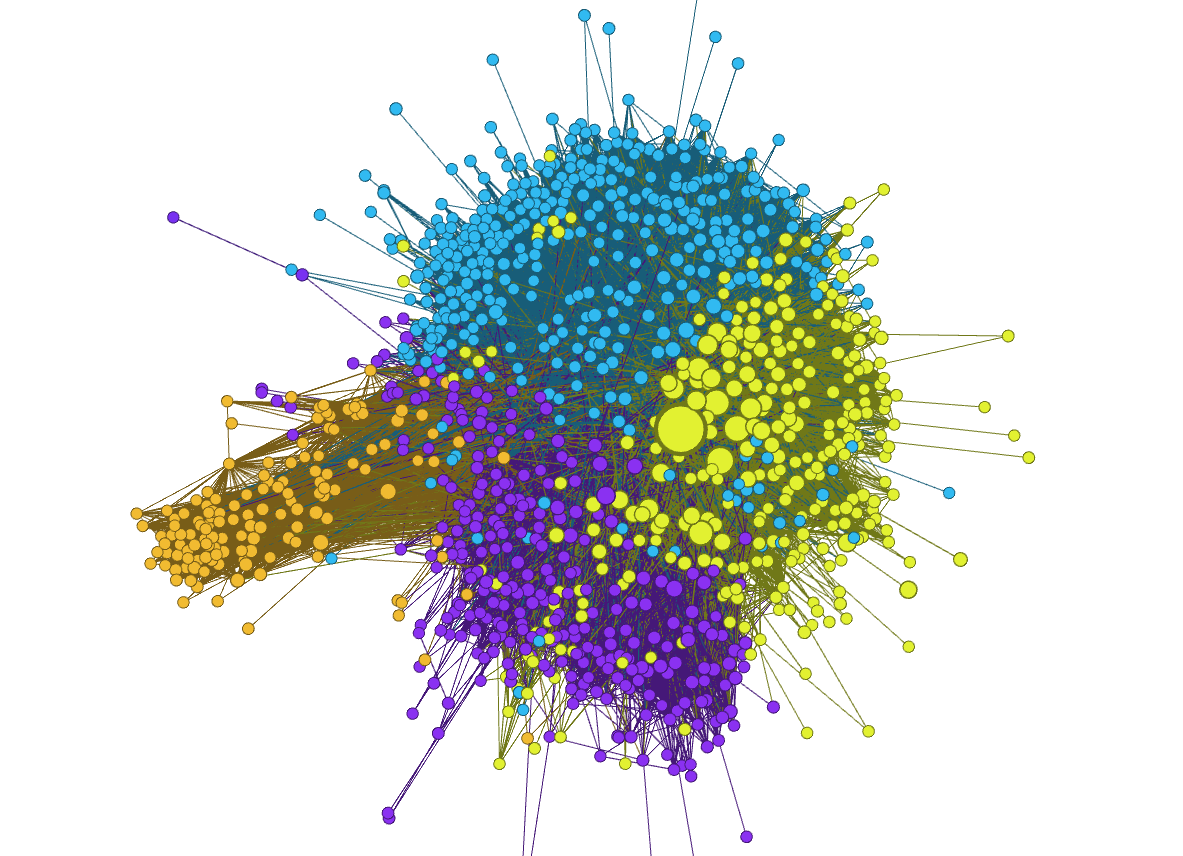
\includegraphics[width=0.9\textwidth]{Y13Q2_community.png}
    \label{fig:static_community}
  }
  \subfigure[Dataset Y13Q2, coloured with Languages Used by Repositories] { 
    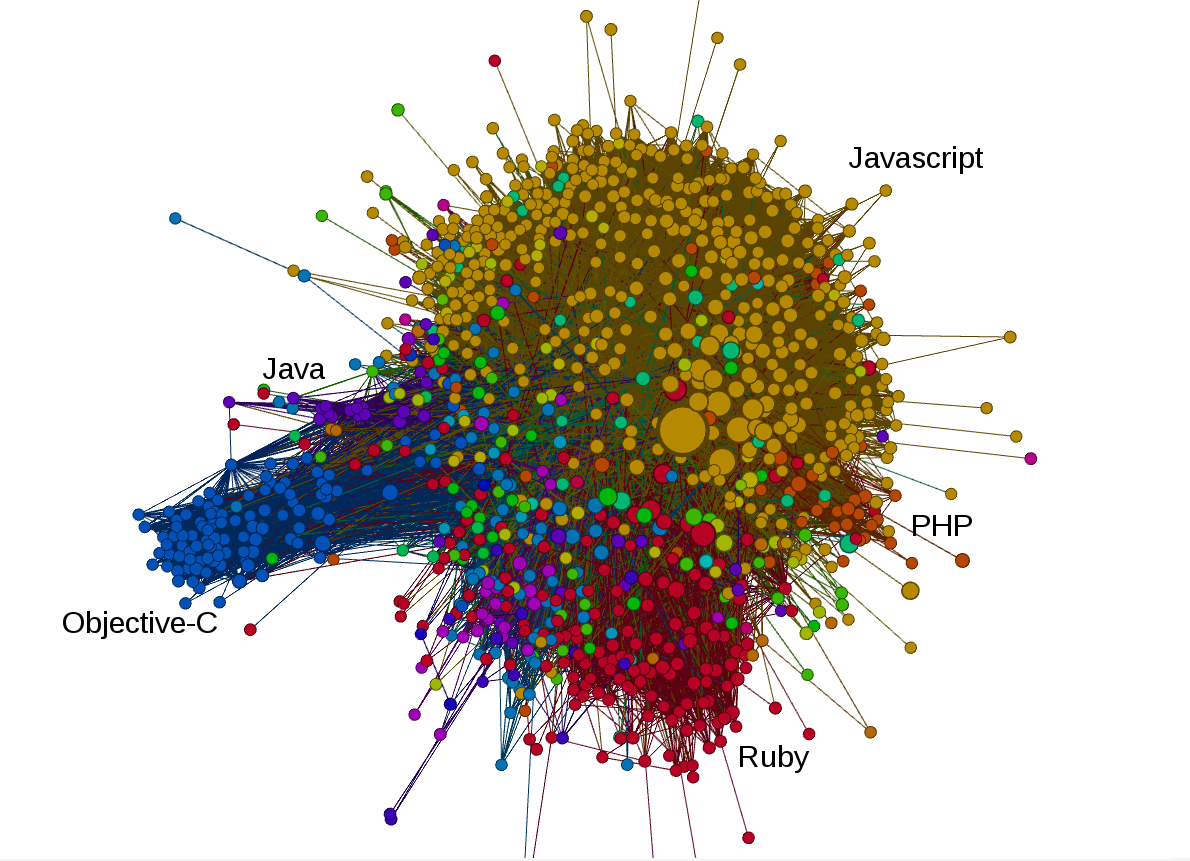
\includegraphics[width=0.9\textwidth]{Y13Q2_lang.png}
    \label{fig:static_lang}
  }
  \caption{Dataset Y13Q2, Colouring with community and language}
\end{figure}

\begin{figure}[htp!]
  \begin{center}
    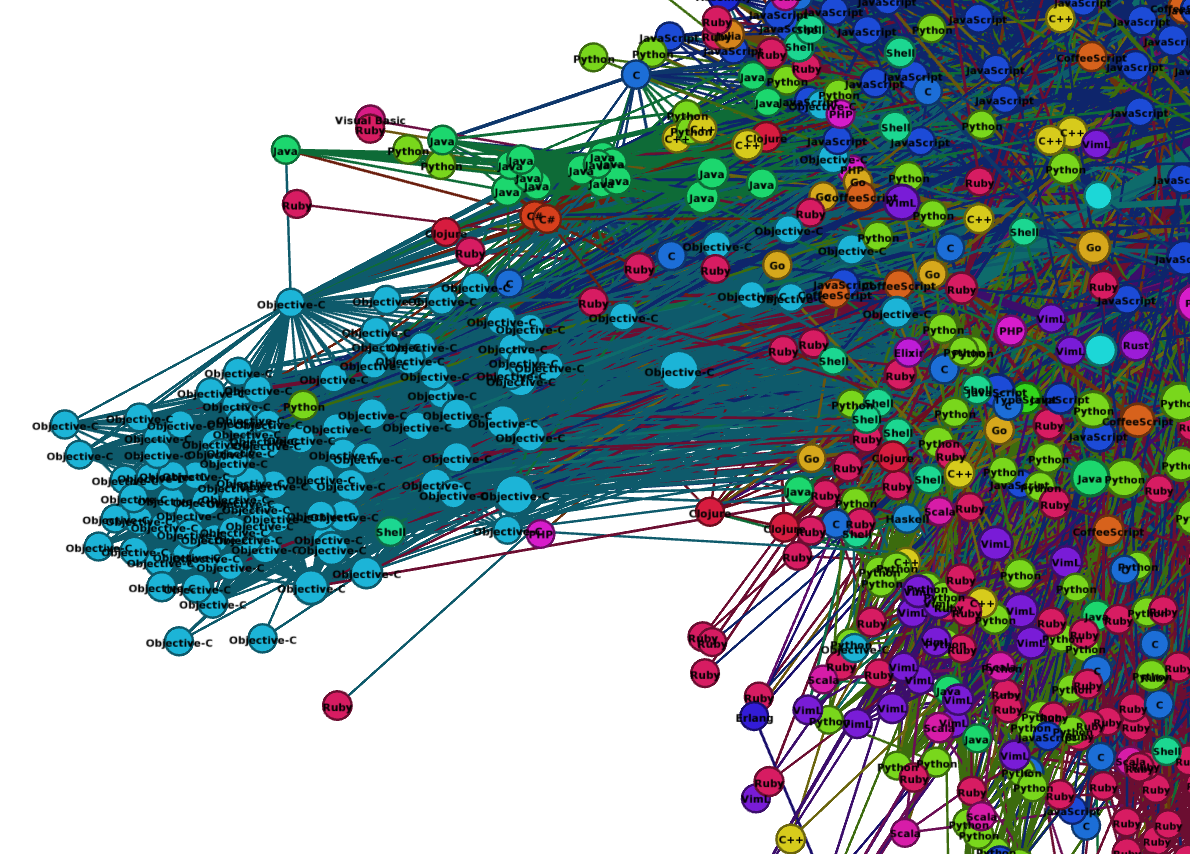
\includegraphics[width=0.9\textwidth]{Y13Q2_zoom.png}
  \end{center}
  \caption{Dataset Y13Q2, Zoomed into Objective-C cluster}
  \label{fig:zoom_2013}
\end{figure}



\subsubsection{Analysis of Network Metrics}
To deeper understand the Y13Q2 dataset, degrees (weighted and unweighted) as well as betweenness (weighted and unweighted) are caculated and the top 10 repositories of each metrics are shown in tables \ref{tab:unweight_degree}, \ref{tab:weight_degree}, \ref{tab:unweight_between}, \ref{tab:weight_between}.

In terms of the degrees, it can be seen that Javascript repositories are likely to be "common interests" of many users, because degrees, weighted or not, generally shows how commonly the repository is starred by users along with other repositories. And weighted degrees may better show the popularity amongst the users, while degree more focuses on the inter-repository relationship.

In fact, the observed phenomenon is reasonable when considering the real situation: 1) Javascript is an easy-to-get-started language with relatively flat learning curve, thus liked or touched by many users from different fields; 2) The number of Javascript repositories that have over 1000 stars is already high, and people are likely to be interested in the language they know.

However, when comparing top-degree repositories with top-star repositories, it turns out that repositories with high star number may not necessarily be the top-degree repository. For instance, twitter/bootstrap has the highest star number (52333), whereas yui/pure only has 4231 stars, but it is shown twitter/bootstrap is not as common-liked as yui/pure, and several other repositories. This phenomenon may be due to temporal factors. For example, twitter/bootstrap is a long-published repository while yui/pure is much younger than twitter/boostrap. Also the name of twitter may attract more people since it is a very popular platform, while yui, an open-source Javascript and CSS library, is less well-known to common people.

While in terms of the betweenness, in particular the weighted betweenness, the top repositories tend to be useful utilities, therefore more popular amongst people who use different languages. For instance, the unconed/TermKit is a terminal / command application, github/gitignore a collection of .gitignore templates, and progrium/localtunnel a local-sever-to-internet exposer, all share the same feature that they can be useful to any programmer or GitHub user. And actually, this phenomenon well collaborate with the meaning of betweenness centrality.

\begin{table}[ht]
  \scriptsize
  \centering
  \begin{minipage}[b]{0.45\linewidth}
    \centering
    \begin{tabular}{cc}
      Repositories        & Degrees \\
      \hline
      yui/pure            & 1252 \\
      heelhook/chardin.js & 1239 \\
      topcoat/topcoat     & 1235 \\
      angular/angular.js  & 1233 \\
      dypsilon/frontend-dev-bookmarks & 1232 \\
      hakimel/Ladda       & 1231 \\
      jakiestfu/Snap.js   & 1230 \\
      FortAwesome/Font-Awesome & 1229 \\
      zmoazeni/csscss     & 1228 \\
      twitter/bootstrap   & 1227 \\
      \hline
    \end{tabular}
    \caption{Unweighted Degrees}
    \label{tab:unweight_degree}
  \end{minipage} %
  \hfill %
  \begin{minipage}[b]{0.45\linewidth}
    \centering
    \begin{tabular}{cc}
      Repositories        & Degrees \\
      \hline
      yui/pure            & 49033 \\
      heelhook/chardin.js & 39376 \\
      hakimel/Ladda       & 38779 \\
      topcoat/topcoat     & 35796 \\
      dypsilon/frontend-dev-bookmarks & 35491 \\
      jakiestfu/Snap.js   & 34491 \\
      helios-framework/helios & 30749 \\
      angular/angular.js  & 30733 \\
      twitter/bootstrap   & 30589 \\
      dimsemenov/Magnific-Popup & 30114 \\
      \hline
    \end{tabular}
    \caption{Weighted Degrees}
    \label{tab:weight_degree}
  \end{minipage}

  \begin{minipage}[b]{0.45\linewidth}
    \centering
    \begin{tabular}{cc}
      Repositories        & Betweenness \\
      \hline
      yui/pure            & 3020 \\
      angular/angular.js  & 2605 \\
      gitlabhq/gitlabhq   & 2553 \\
      h5bp/html5-boilerplate & 2494 \\
      github/gitignore    & 2331 \\
      mneorr/Alcatraz     & 2327 \\
      heelhook/chardin.js & 2305 \\
      toursprung/TSMessages & 2149 \\
      usablica/intro.js   & 2146 \\
      designmodo/Flat-UI  & 2077 \\
      \hline
    \end{tabular}
    \caption{Unweighted Betweenness}
    \label{tab:unweight_between}
  \end{minipage} %
  \hfill %
  \begin{minipage}[b]{0.45\linewidth}
    \centering
    \begin{tabular}{cc}
      Repositories        & Betweenness \\
      \hline
      unconed/TermKit     & 2093 \\
      gotosleep/JASidePanels & 1945 \\
      progrium/localtunnel & 1755 \\
      usablica/intro.js   & 1621 \\
      github/gitignore    & 1618 \\
      sobri909/MGBox2     & 1562 \\
      square/crossfilter  & 1559 \\
      tonymillion/Reachability & 1552 \\
      Simbul/baker        & 1536 \\
      mneorr/Alcatraz     & 1531 \\
      \hline
    \end{tabular}
    \caption{Weighted Betweenness}
    \label{tab:weight_between}
  \end{minipage} %
\end{table}

\subsection{Dynamic Analysis}
\subsubsection{Visual Observation}

Figures \ref{fig:dyn_comm} and \ref{fig:dyn_lang} are present to show the general trend of GitHub repository interest graph evolution over time.
It can be seen that generally, language and community are closely correlated over all the time, not only for Y13Q2 data as analyzed previously.

Also, as time goes by, the number of language clustering is as well increasing -- from Y12Q2 with ~3 big clusters, to Y14Q2 with ~6 clusters. 
And this process is actually a gradual evolution, for example, Java cluster was almost un-obsevable in Y12Q2, and a small cluster was established near Objective-C in Y13Q2, and in Y14Q2, the Java cluster already forms another out-standing cluster just as Objective-C cluster -- they form two sharp strikes in the graph plot, as shown in figure \ref{fig:zoom_java_2014}. 

This increase of language cluster possibly shows that GitHub is actually getting more and more popular among programmers using different languages. And they are increasingly likely to share their codes and get aquainted with other people's work on GitHub.


Diving into the Y14Q2 language, we can still find out that the largest community or language cluster is still Javascript. However, as is shown in a zoomed version in figure \ref{fig:zoom_js_2014}, there are many red dots inside the Javascript cluster, which are CSS repositories. 

After taking a deeper investigation, two factors may be contributing to this phenomenon: 
1) these CSS repositories are indeed using CSS as its highest portion of languages used, while Javascript usually just lies next to CSS, therefore the repositories still is highly relying on Javascript; 2) GitHub may have enhanced their language detection routines to seperate CSS from Javascript after Y13Q2, because from the data, it is strange that neither Y13Q2 nor Y12Q2 has CSS repositories included.

\begin{figure}[htp!]
  \subfigure[Y12Q2]{ %
    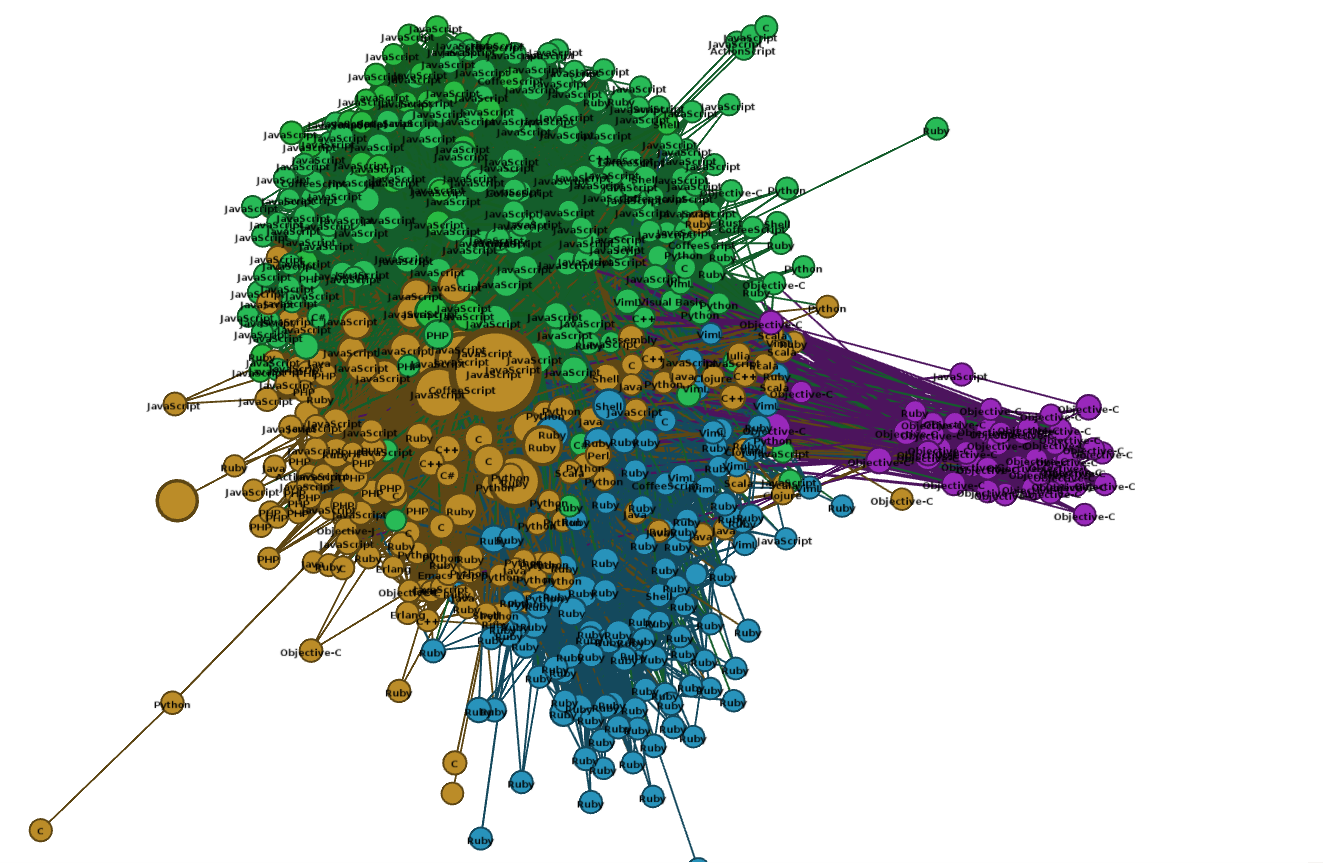
\includegraphics[width=0.3\textwidth]{Y12Q2_comm.png} %
  } %
  \subfigure[Y13Q2]{ %
    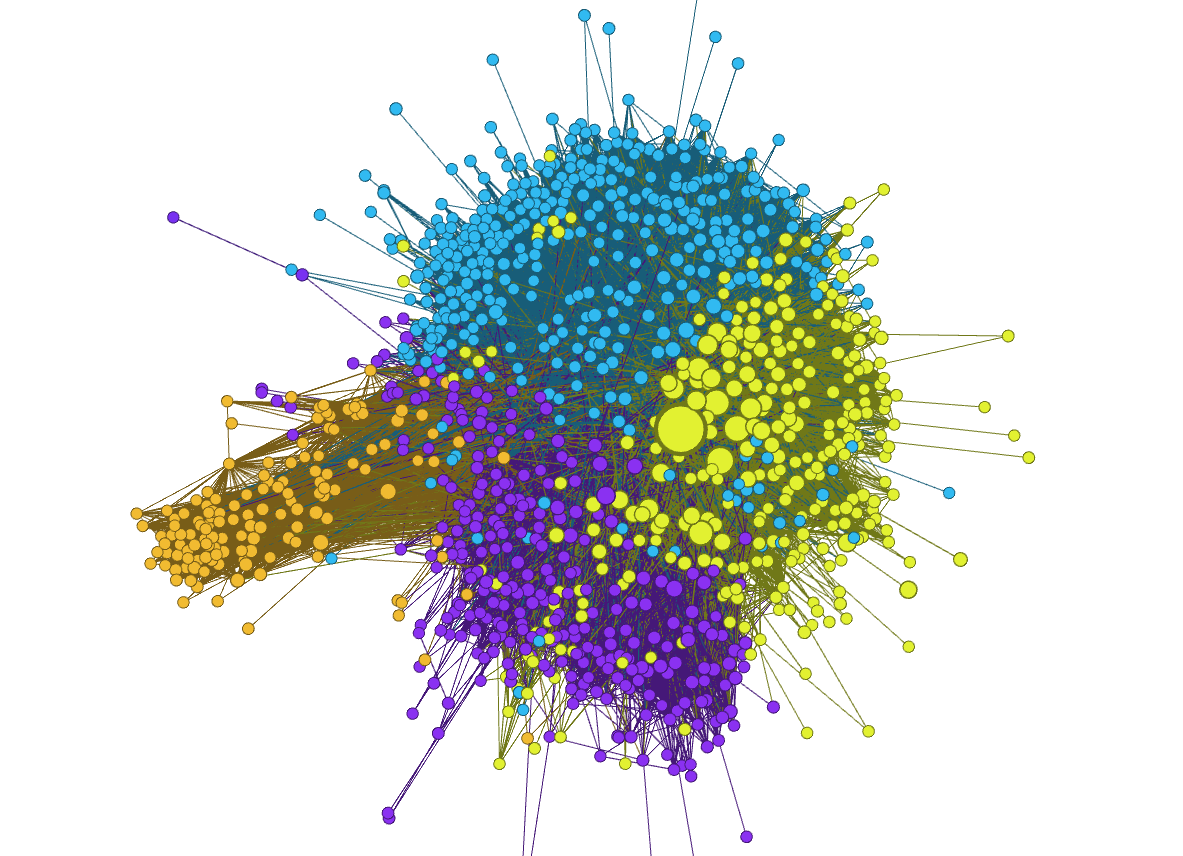
\includegraphics[width=0.3\textwidth]{Y13Q2_comm.png} %
  } %
  \subfigure[Y14Q2]{ %
    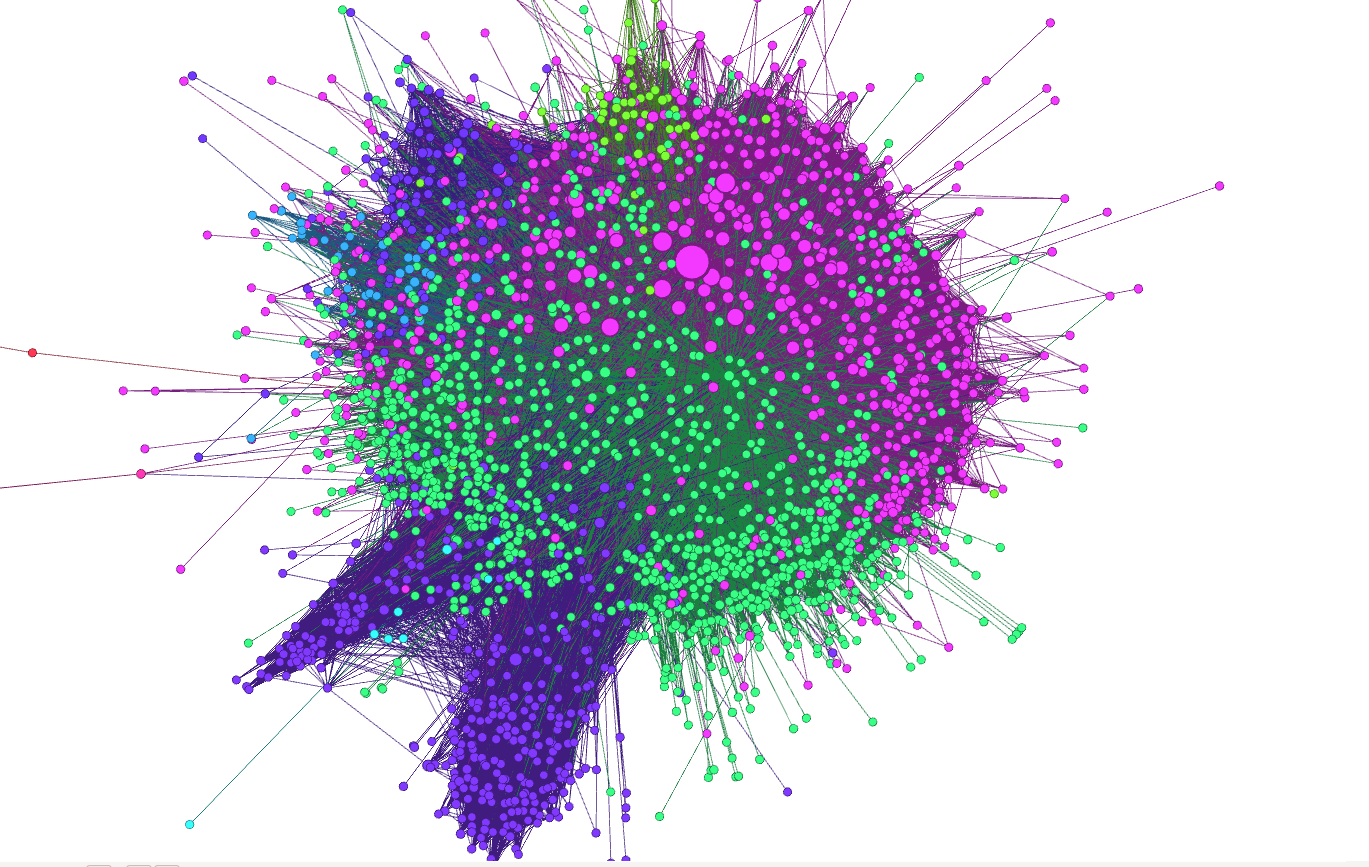
\includegraphics[width=0.3\textwidth]{Y14Q2_comm.png} %
  }
  \caption{Community Colouring Graphs}
  \label{fig:dyn_comm}

  \subfigure[Y12Q2]{ %
    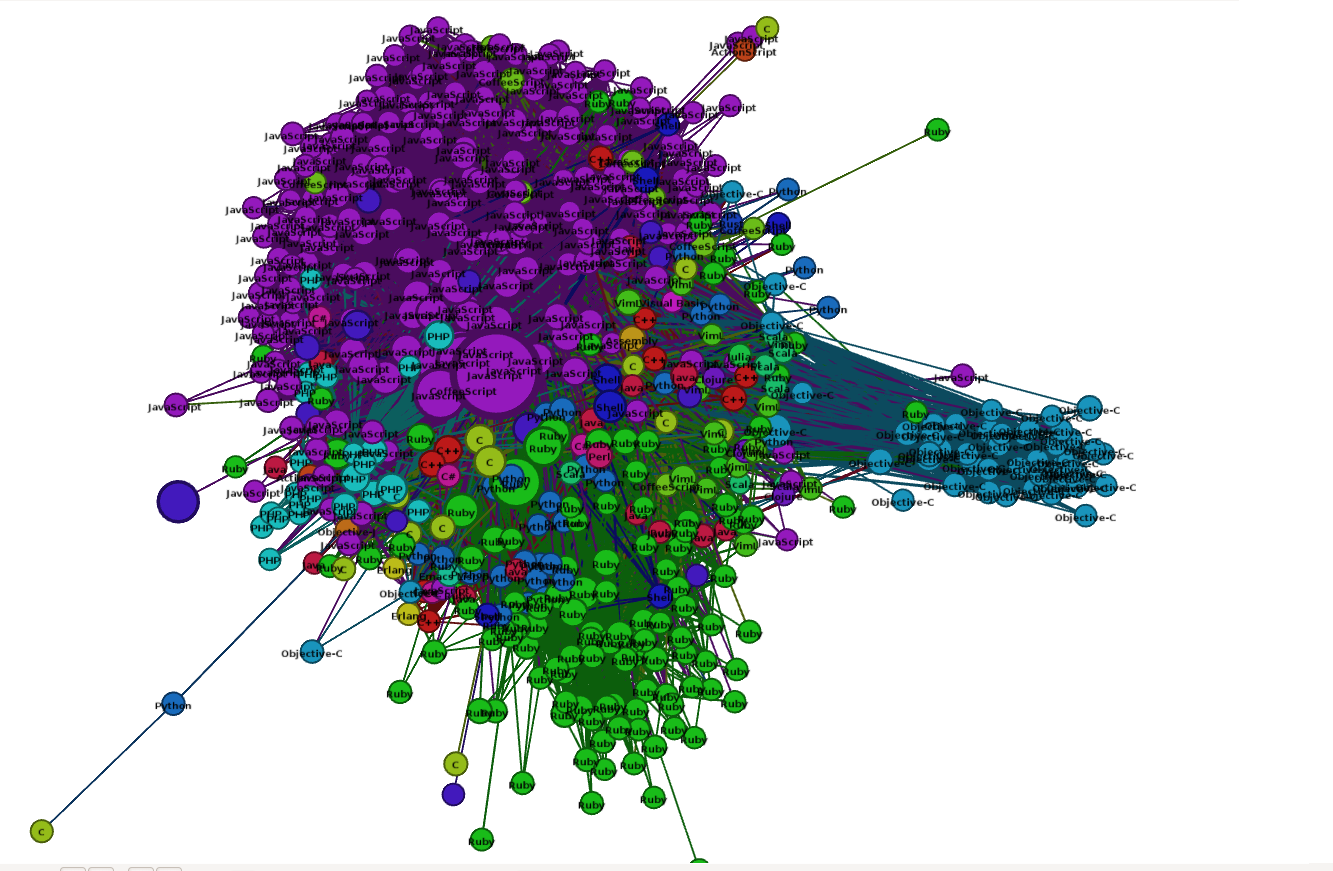
\includegraphics[width=0.3\textwidth]{Y12Q2_lang.png} %
  } %
  \subfigure[Y13Q2]{ %
    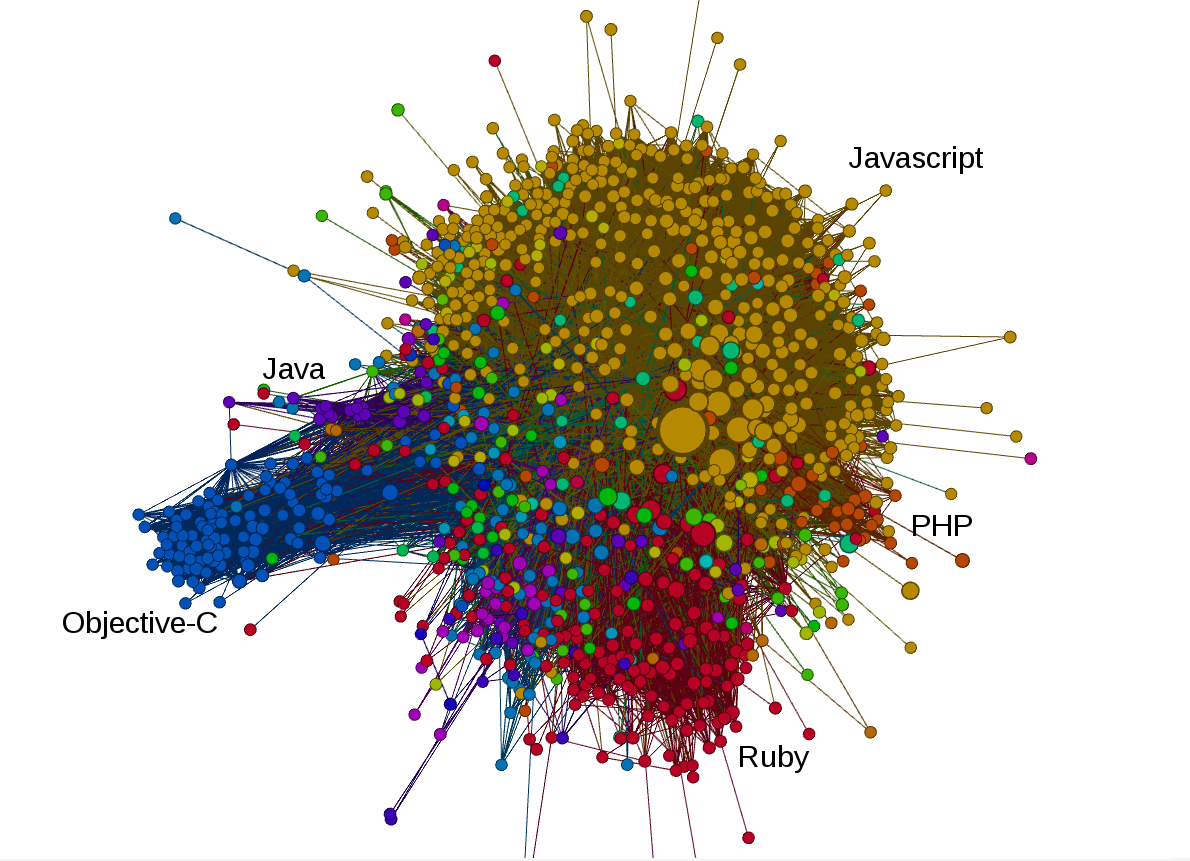
\includegraphics[width=0.3\textwidth]{Y13Q2_lang.png} %
  } %
  \subfigure[Y14Q2]{ %
    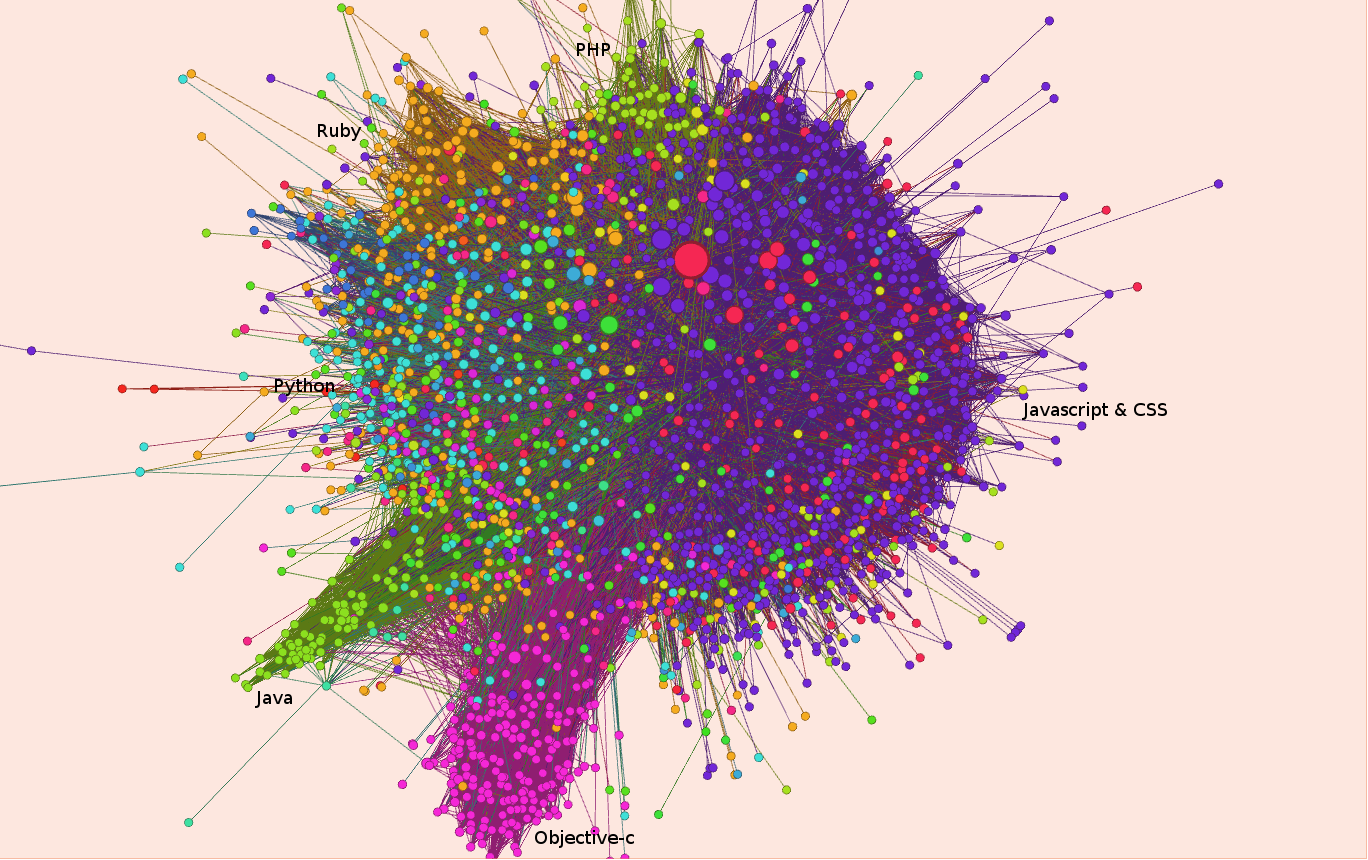
\includegraphics[width=0.3\textwidth]{Y14Q2_lang.png} %
  }
  \caption{Language Colouring Graphs}
  \label{fig:dyn_lang}
\end{figure}

\begin{figure}[htp!]
  \centering
  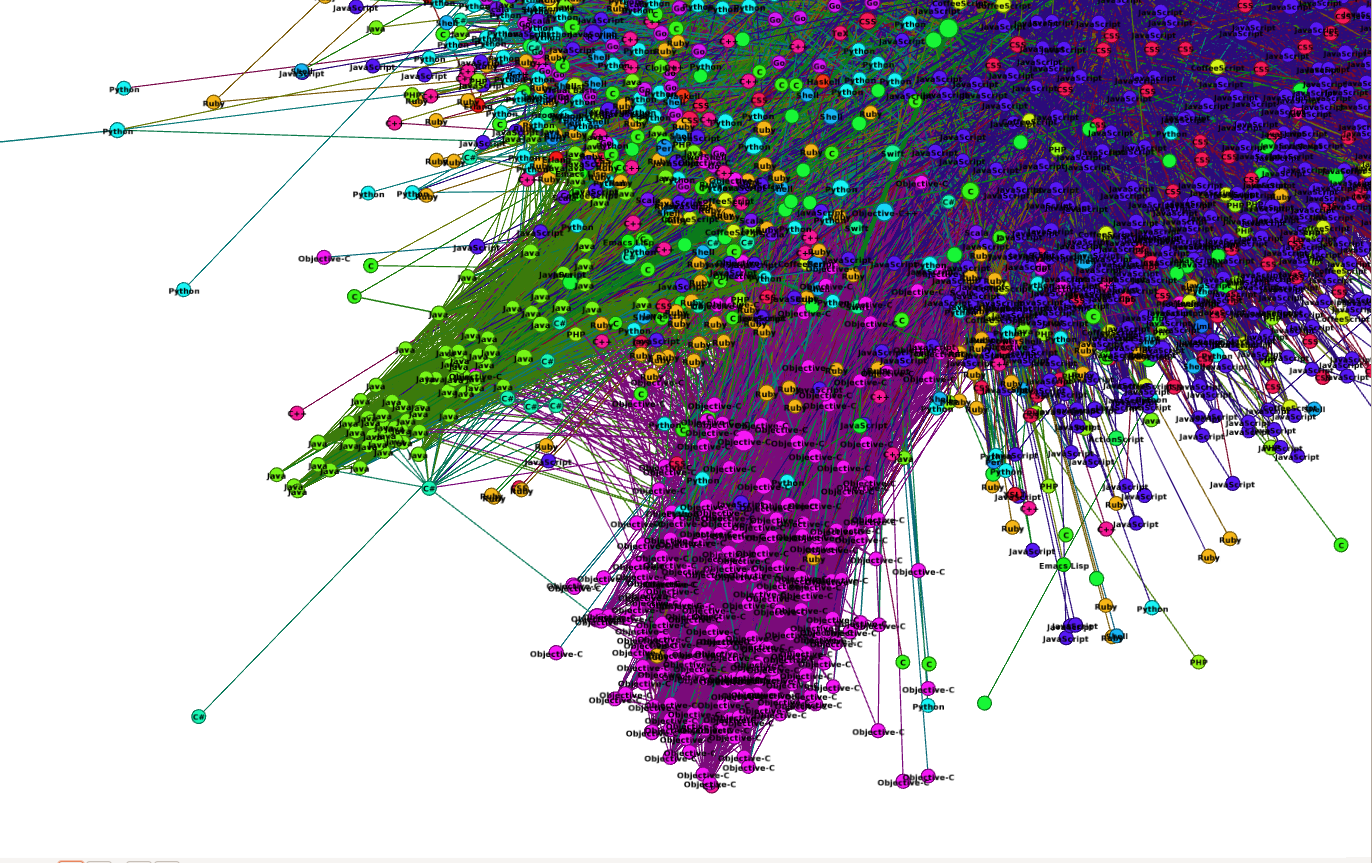
\includegraphics[width=0.9\textwidth]{Y14Q2_lang_zoom_java.png} %
  \caption{Y14Q2 Zoomed Version of Language Colouring Graph -- Java and Objective-C}
  \label{fig:zoom_java_2014}
\end{figure}

\begin{figure}[htp!]
  \centering
  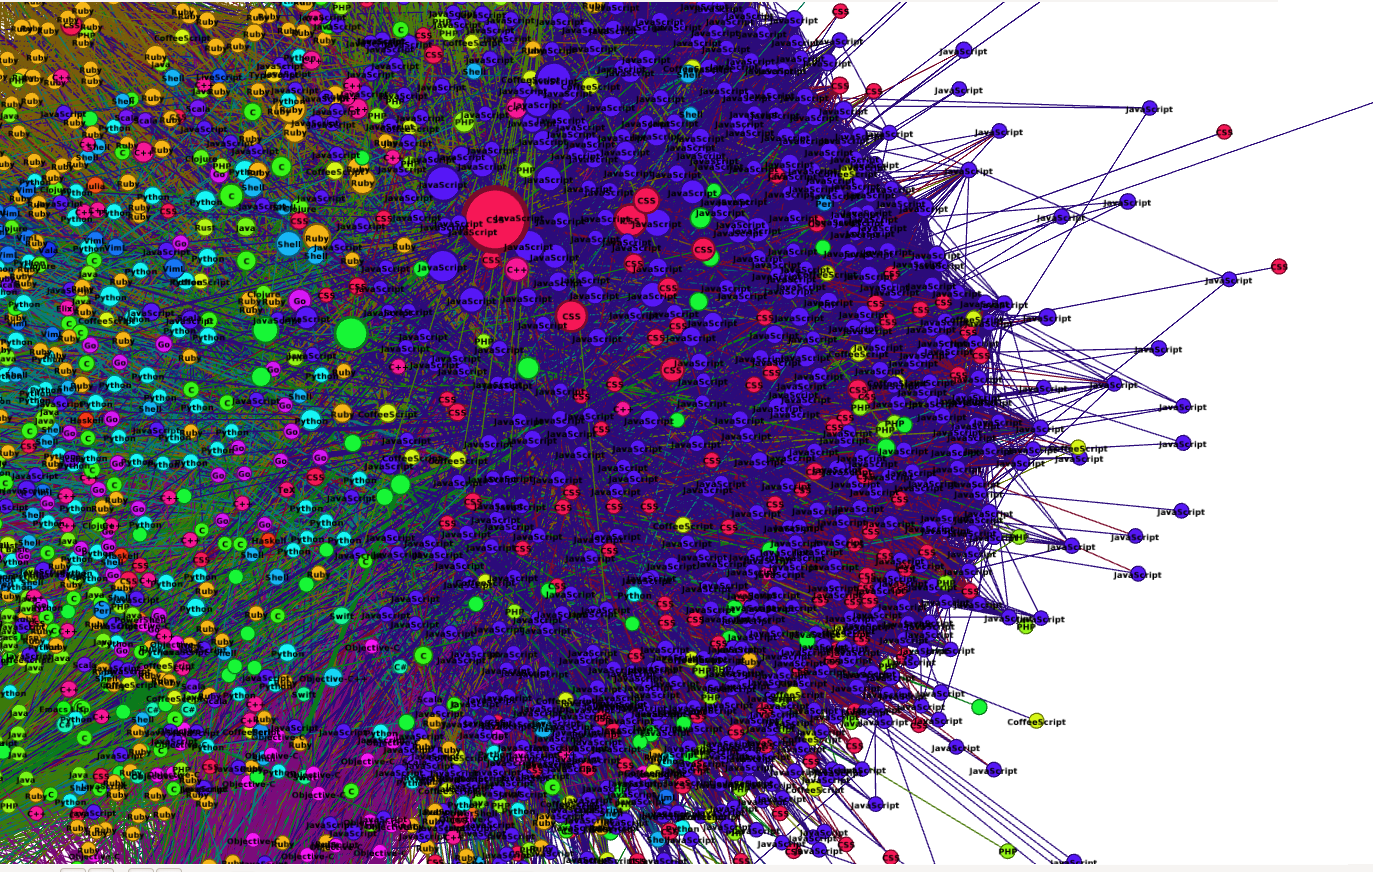
\includegraphics[width=0.9\textwidth]{Y14Q2_lang_zoom_js.png} %
  \caption{Y14Q2 Zoomed Version of Language Colouring Graph -- Javascript}
  \label{fig:zoom_js_2014}
\end{figure}

\subsubsection{Analysis of Network Metrics}
To quantatively analyze the network change, we caculated average path length and density of 11 graph snapshots, as well as the node and edge count trend, shown in figure \ref{fig:trend}.

From the plots of average path length and density, it is hard to conclude any increasing or decreasing trend. Rather, the general trend looks to be scattering around a certain value.

However, when looking into the node and edge count trends, it is obvious to tell a linear or polynomial increase.

Therefore, it shows that for the GitHub repository interest graph, although it increases in size quickly throughout time, the density or average path length is not remarkably increased. That is, repositories are almostly as tightly connected to each other as before, based on the context of users' interest, and therefore users of GitHub are possibly diverse in interest, as well as the repositories.

Also, when focusing on certain repositories' weighted degree, it can also be found that some repositories were popular once but then tend to be unknown, while others may be continuously popular among people, though the starring people of each quarter may not be that many.

For instance, in Y14Q1, there is a repository naming sahat/hackathon-starter. It achieved a 83571 weighted degree at that time, ranking the first amongst 2180 repositories of interest. However, in Y14Q3, it only obtained 5447 weighted degree. Although still relatively high, its great days are no more -- it's ranking 430 out of 2998 repositories.

In contrast, repository twbs/bootstrap achieved 35419 weighted degree in Y14Q1, ranking 44, and still has 32198 weighted degrees in Y14Q3, ranking 67.

Therefore, different repositories have different popularity trend from this observation.

\begin{figure}[htp!]
  \centering
  \subfigure[Average Path Length]{ %
    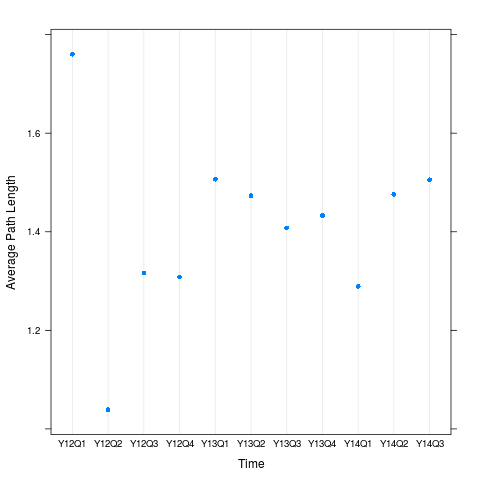
\includegraphics[width=0.45\textwidth]{apl.png} %
  } %
  \subfigure[Density]{ %
    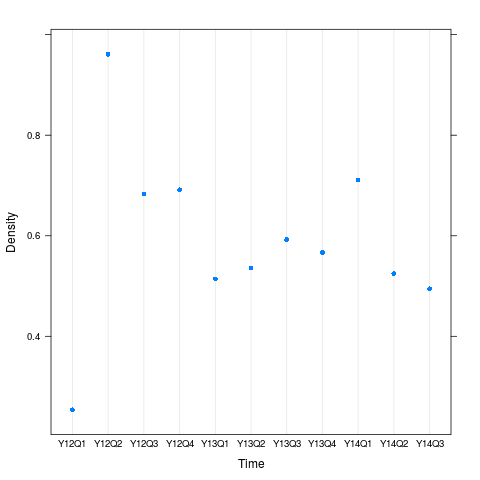
\includegraphics[width=0.45\textwidth]{density.png} %
  }
  \subfigure[Node Count]{ %
    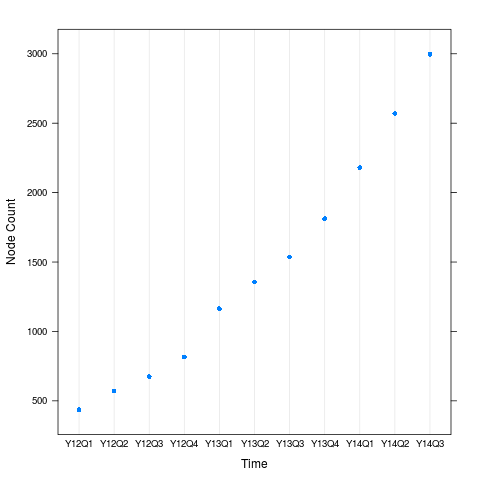
\includegraphics[width=0.45\textwidth]{node.png} %
  } %
  \subfigure[Edge Count]{ %
    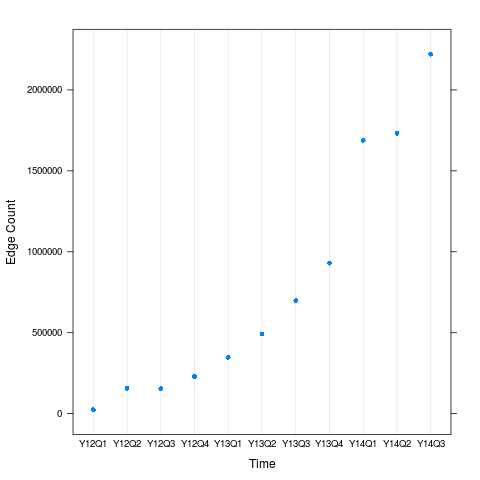
\includegraphics[width=0.45\textwidth]{edge.png} %
  }
  \caption{Network Metrics Trend}
  \label{fig:trend}
\end{figure}

\section{Conclusion}

In this paper, analysis is made to explore, on GitHub, how users' interest towards repositories are like, how repositories are related based on such context, and how such relationship may evolve over time.

The conclusion, based on both visual observations and network metrics analysis, is:
\begin{enumerate}
\item users tend to be interested in the repositories of the languages they are familiar with;
\item repositories of same languages or languages of the same function are likely to be clustered together;
\item over time, more and more users with different language preferences are likely to migrate into GitHub, thus creating more and more language communities, exposing clearer language community characteristics;
\item over time, the repository interest graph is increasing in size, but its density, i.e. inter-repository relationship, tends to keep tight;
\item over time, some repositories got really high popularity but later falls into less known, while some continuously have mild starring number.
\end{enumerate}

However, since the data sampled are only limited to repositories with high star number, the conclustions made in this work may not be accurate, for even more repositories, which may be popular among smaller groups, are not included into the examination. Further work need to be done if a deeper investigation is to be made.
Also, starring is only one aspect showing users' interests, whereas forking, watching, user following are also essential to be applied for analysis. The data used in this work is therefore limited to certain extent. More comparisons may be needed to better analyze the GitHub network.

\section{Acknowledgement}

This paper is developed as a course project on social network analysis\cite{snacourse}.
All source codes as well as plots are available at \url{https://github.com/jiachengpan/sna}.

{\small
\bibliographystyle{plain}
\bibliography{report}
}

\end{document}

